%% Kiii-Kiii — SAC 2027 AIFT independent submission draft
%% Submission: anonymous sigconf; target <=8 total pages including references.
%% Camera-ready: \documentclass[sigconf]{acmart} and remove \anonv
\documentclass[sigconf,anonymous]{acmart}

\usepackage{booktabs}
\usepackage{tabularx}
\usepackage{ragged2e}
\usepackage{xurl}           % Allow long schema labels and URLs to wrap.
\usepackage{xcolor}
\usepackage{kotex}          % Korean examples in text; comment out if Overleaf compiler lacks kotex (use xelatex/lualatex)
% Keep Hangul upright within Latin emphasis: these fonts have no italic face.
\setmainhangulfont{UnBatang.ttf}[
  BoldFont=UnBatangBold.ttf,
  ItalicFont=UnBatang.ttf,
  BoldItalicFont=UnBatangBold.ttf,
  Script=Hangul,Language=Korean]
\usepackage{enumitem}
\setlist{nosep,leftmargin=*}
% A last-pass line-breaking allowance for narrow columns; no changes to
% ACM margins, type sizes, line spacing, or paragraph spacing.
\setlength{\emergencystretch}{2em}

%% --- anonymisation helpers: \anonv{visible}{hidden} shows the first arg in review mode
\newif\ifanonymous\anonymoustrue
\newcommand{\anonv}[2]{\ifanonymous#1\else#2\fi}   % acmart already defines \anon; ours is \anonv{visible-in-review}{camera-ready}
\newcommand{\todo}[1]{\textcolor{red}{[TODO: #1]}}

%% Anonymous review metadata; final ACM rights metadata supplied after acceptance.
\setcopyright{none}
\copyrightyear{2027}
\acmYear{2027}
\acmDOI{}
\acmISBN{}
\acmConference[SAC '27]{The 42nd ACM/SIGAPP Symposium on Applied Computing}{April 5--9, 2027}{Gwangju, South Korea}
\settopmatter{printacmref=false}
\renewcommand\footnotetextcopyrightpermission[1]{}

\begin{document}



%% Name: \kiii = Kiii^2 (= "Kiii Kiii"). Backronym K-I-I-I = Korean / Identifiers (Tier L) / Identifiability (Tier I) / Ill-formed inputs (variation axis)
\newcommand{\kiii}{Kiii\textsuperscript{2}}
%% Title spells the name "Kiii-Kiii" (after the girl group); body text uses \kiii (= Kiii^2) for the dataset.
\title[Kiii-Kiii: Korean Financial PII Detection]{Kiii-Kiii: Korean Identifiers, Identifiability, and Ill-formed Inputs}
\subtitle{A Regulation-Grounded Benchmark for Financial PII Detection}
%% alternatives kept for the record:
%%  Kiii^2: Benchmarking Korean Financial PII across Identifiers, Identifiability, and Irregular Surface Forms
%%  Korean Financial PII under Imperfect Inputs: an Identifiability-Aware Benchmark for AI DLP (Kiii^2)

\begin{abstract}
Financial privacy evaluation must specify what to detect as well as how it appears in text. Korean financial documents---including call-center transcripts and scanned forms---combine jurisdiction-specific categories, noncanonical identifiers and contextual attributes. Recognizing a standard identifier pattern therefore addresses only part of the task. We introduce \textbf{Kiii-Kiii} (dataset \kiii{}), a benchmark that makes these dimensions explicit. A 36-category taxonomy distinguishes 24 categories with statutory grounds from 12 additional quasi-identifier and profiling categories, without equating detection with a legal duty to redact. The synthetic preview contains 1,440 documents and 218,664 spans across ten document types, with code-generated identifiers, applicable checksum checks and four levels of surface-form variation. A matched full-context versus local-window protocol holds target regions and output budgets fixed, enabling analysis of whether additional context improves span recovery. Exact span scoring retains malformed and truncated responses as failures. Across 12 language models and three frozen baselines, strict extraction is limited by both output-contract failures and missed spans. A fixed, post-hoc itemwise parser provides a closer observable proxy for detection, reaching 31.58 F1 while retaining all gold and penalizing invalid items. Local context improves this diagnostic in all ten completed paired comparisons; strict scores favor local in nine. These findings motivate separate reporting of extraction reliability and detectable span recovery. The preview is released under CC BY-NC 4.0, with a formal release to follow.

\end{abstract}

\begin{CCSXML}
<ccs2012>
<concept><concept_id>10002978.10003029</concept_id><concept_desc>Security and privacy~Human and societal aspects of security and privacy</concept_desc><concept_significance>500</concept_significance></concept>
<concept><concept_id>10010147.10010178.10010179</concept_id><concept_desc>Computing methodologies~Natural language processing</concept_desc><concept_significance>300</concept_significance></concept>
</ccs2012>
\end{CCSXML}
\ccsdesc[500]{Security and privacy~Human and societal aspects of security and privacy}
\ccsdesc[300]{Computing methodologies~Natural language processing}
\keywords{PII detection, Korean financial NLP, regulation-grounded benchmark, long-context extraction, output reliability}

\maketitle

\section{Introduction}
\label{sec:intro}

\begin{figure*}[t]
\centering
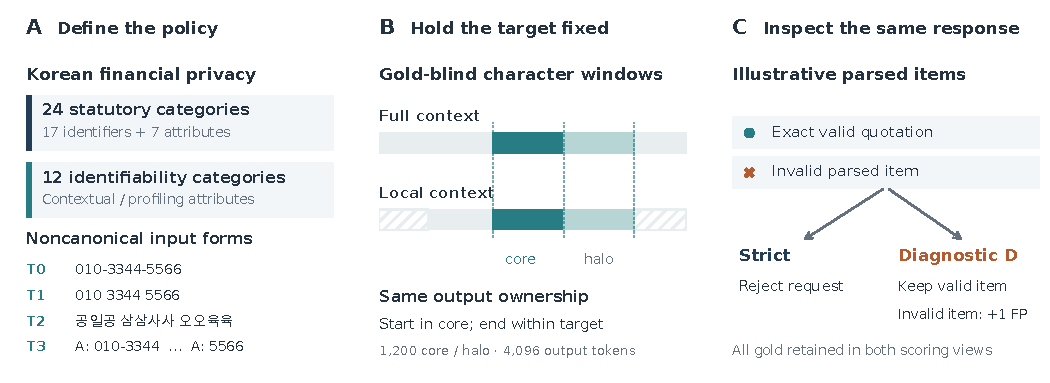
\includegraphics[width=\textwidth]{figures/benchmark-overview.pdf}
\caption{\textbf{From detection policy to an auditable extraction task.}
(A) The 36-category policy and illustrative T0--T3 forms of one synthetic
identifier. (B) Full and local context share core ownership, a following
halo and the output budget; the schematic is not to scale. (C) An illustrative
normally completed response with one valid and one invalid parsed item:
strict scoring rejects the request, while D retains the valid item and
charges an invalid-item false positive. Both retain all gold. This example
explains the scoring contract, not a causal partition of model ability.}
\Description{Three panels connect the 24 statutory and 12 identifiability
categories, a matched full/local context window, and strict versus itemwise
validation of the same received response. Korean digit words and split turns
illustrate noncanonical synthetic identifier forms.}
\label{fig:overview}
\end{figure*}


Recognizing a well-formed identifier is only one part of detecting personal information in financial text. A customer may dictate an account number as \textup{일일공 에 일이삼 에 사오육칠팔구}, split it across turns, or provide a partially masked value. A repayment difficulty or an upcoming life event can also convey personal information without resembling an identifier. A benchmark for data loss prevention (DLP) must therefore make both the detection policy and the conditions of recognition explicit.

Korean finance brings these requirements together. Statutory categories include customer identifiers and financial attributes beyond conventional name--address--phone labels (\S\ref{sec:taxonomy}). Some additional attributes are useful to study because they can support profiling~\cite{staab2024beyond}, even when they are not separately enumerated in our statutory mapping. Treating all such targets as an undifferentiated PII label obscures what a detector covers; treating all detected spans as legally requiring redaction conflates evaluation policy with legal obligation.

Document context introduces a second ambiguity. Surrounding text may establish that an amount or statement concerns a person, but a long record may also contain unrelated details and multiple customers. Moreover, accepting a long input does not ensure that a model can enumerate all sensitive spans within a finite response. Full-document and chunked extraction are difficult to compare when they also change the amount of output requested. This motivates our central question: \emph{under an explicit Korean financial detection policy and a fixed output task, how does access to wider context affect recovery of identifiers and contextual attributes across input variations?}

Existing work studies query-aware PII protection~\cite{shen2025piibench}, multilingual detection~\cite{vats2026redact}, Korean dialogues~\cite{fei2024kdpii} and court judgments~\cite{hahm2025thunderdeid}. Korean financial benchmarks additionally establish the value of domain-specific evaluation~\cite{hwang2025twice,lee2025nmixx}. \kiii{} connects these directions through a shared taxonomy, controlled input variation and a matched context comparison. We contribute:
\begin{enumerate}
  \item \textbf{An auditable detection policy:} 36 categories separating statutory grounds (24) from additional identifiability concerns (12), with category definitions and masking metadata kept distinct (\S\ref{sec:taxonomy}).
  \item \textbf{A controlled financial testbed:} 1,440 synthetic documents and 218,664 spans covering ten document types, multiple subjects and T0--T3 variation, with code-generated identifiers and span-level provenance (\S\ref{sec:benchmark}).
  \item \textbf{A matched context evaluation:} full-document and local-window inputs applied to identical target regions and output budgets, across 12 language models and three frozen baselines, with explicit failure accounting (\S\ref{sec:setup}). Archived-response diagnostics separate output compliance, grounding errors and observable detection, revealing why strict extraction scores alone can conceal useful span recovery.
\end{enumerate}

\section{Related Work}
\label{sec:related}

\paragraph{PII detection and anonymization.}
PII-Bench~\cite{shen2025piibench} evaluates query-aware privacy protection, including multi-subject settings. REDACT~\cite{vats2026redact} organizes multilingual detection by sensitivity and disclosure form, while Mind the Gap~\cite{zafar2026mindthegap} examines distribution shifts. These works motivate evaluation beyond canonical entity recognition. \kiii{} focuses on Korean financial categories and input transformations under a shared operational policy. The Text Anonymization Benchmark~\cite{pilan2022tab} distinguishes direct and quasi-identifiers and evaluates disclosure risk. Anonymization systems~\cite{staab2025anonymizers,yang2025rupta} and re-identification benchmarks~\cite{krco2026ratbench} address privacy--utility trade-offs. Our task is narrower: exact recovery of typed spans, without claiming that extraction F1 measures residual disclosure risk or anonymization quality.

\paragraph{Korean PII.}
KDPII~\cite{fei2024kdpii} studies de-identification in Korean dialogues; Jang et al.~\cite{jang2024koreanpiiner} develop a Korean personal-information recognizer. Thunder-DeID~\cite{hahm2025thunderdeid} provides a detailed taxonomy for court judgments. These resources establish Korean PII detection as a distinct evaluation setting. We complement them with explicit financial category mappings, recorded surface-form operations and a fixed-output comparison of document context. This scope differs from conversational text anonymization~\cite{albanese2026anonymous} and from contextual privacy judgments about appropriate disclosure~\cite{mireshghallah2024confaide,shao2024privacylens}.

\paragraph{Korean financial language evaluation.}
TWICE~\cite{hwang2025twice} introduces KorFinMTEB for Korean financial embedding evaluation. NMIXX~\cite{lee2025nmixx} studies Korean--English financial embeddings and introduces KorFinSTS. KFinEval-Pilot~\cite{hwang2025kfineval} evaluates financial knowledge, legal reasoning and toxicity; KRX Bench~\cite{son2024krx} evaluates company knowledge across markets. \kiii{} extends this domain-specific evaluation agenda to privacy detection: recovering which text spans fall under an explicit policy, rather than measuring financial knowledge or semantic similarity.


\section{Taxonomy}
\label{sec:taxonomy}

%% ~0.6 page. Table 1 = compact category table. Full statute quotes → appendix / repo.
Our taxonomy has two tiers and two kinds. \textbf{Tier L (Legal)} groups 24 operational categories grounded in Korean statutes and regulations: the Personal Information Protection Act (PIPA) \S23--24 and Enforcement Decree \S18--19 (sensitive and unique identifying information); the Credit Information Act (CIA) \S2 and its Enforcement Decree \S2, which lists 성명·주소·전화번호 (name, address and telephone number), e-mail and SNS addresses, the four national identification numbers, \emph{CI/DI and customer-distinguishing identifiers specified in the Decree} (\S2\,③), and business/corporate registration numbers (\S2\,④); the Real Name Financial Transactions Act \S4 (transaction information); and the Electronic Financial Transactions Act \S2(10) (access media). \textbf{Tier I (Identifiability)} contains additional categories that act as quasi-identifiers~\cite{pilan2022tab} or, when aggregated, enable profiling and personalised social engineering; membership in Tier I is a benchmark design choice, not a claim that these categories lack legal protection.

Each category is an \textbf{identifier} (a name or value used to refer to a person, organization or account) or an \textbf{attribute}. CIA \S2(1)(a) defines identifying information as credit information \emph{only when combined with} transaction, creditworthiness or capacity information; we separately specify a benchmark policy: L-identifiers and sensitive information are \nolinkurl{must_mask}, other L-attributes are \nolinkurl{mask_if_linked}, and Tier I is \nolinkurl{detect_only}. These are operational metadata, not a finding that every occurrence legally requires redaction. Corporate identifiers are retained as financial-record targets, not asserted to identify natural persons. Table~\ref{tab:taxonomy} lists the 36 categories (17 L-identifier, 7 L-attribute, 12 I-attribute). Staff names are annotated as PII with a \nolinkurl{subject_role} of \emph{staff}; institution and product names, biometric templates and unattributed amounts are excluded.

\paragraph{A shared operational policy.}
All 36 categories are scored for every system. Prompted models receive their definitions; baseline labels use frozen mappings. L/I indicates the basis for inclusion, not a sensitivity ranking. Scores measure coverage of this operational policy, not a model's legal or cultural beliefs.

\begin{table}[t]
\caption{Taxonomy overview: all 36 categories, with abbreviated labels. L denotes Legal and I denotes Identifiability.}
\label{tab:taxonomy}
\small
\begin{tabularx}{\columnwidth}{@{}>{\RaggedRight\arraybackslash}p{0.23\columnwidth}>{\RaggedRight\arraybackslash}X@{}}
\toprule
\textbf{Tier / kind} & \textbf{Categories} \\
\midrule
L / identifier\newline (17) & name; RRN; foreigner reg.\ no.; passport; driver's licence; phone; address; e-mail; online handle; customer ID; business reg.\ no.; corporate reg.\ no.; bank account; securities account; card; contract no.; access credential. \\
\addlinespace
L / attribute\newline (7) & credit transaction; transaction record; delinquency; financial capacity; credit score; public record; sensitive information. \\
\addlinespace
I / attribute\newline (12) & DOB/age; gender; nationality; family relation; employer/position; education; life event; investment profile; consultation content; service usage; device/IP; location mention. \\
\bottomrule
\end{tabularx}
\par\smallskip
\begin{minipage}{\columnwidth}
\RaggedRight\small
\textit{Policies.} L identifiers and sensitive information: must mask.
Other L attributes: mask if linked. I attributes: detect only.
Full subtypes, statutory citations and format rules are in the taxonomy specification.
\end{minipage}
\end{table}


\section{Benchmark Construction}
\label{sec:benchmark}

\paragraph{Slot-filling generation.}
We separate identifier generation from document composition to obtain mechanically traceable span offsets. An LLM composes each document from a plan (document type, number of subjects, target length, variation level) using typed slots such as \texttt{\{\{bank\_account\_no:1\}\}} for identifiers and inline tags \texttt{[[credit\_transaction:1]]…[[/…]]} for attribute spans. Code then fills identifier slots with synthetic values, applying supported checksum rules and format templates, records character offsets and entity identity, and rejects documents flagged by its unslotted-identifier checks. Ten financial document types cover forms, transaction records, agreements, transcripts and reports.

\paragraph{Surface-form variation (Figure~\ref{fig:overview}).}
Each document is assigned a level: \textbf{T0} canonical, \textbf{T1} formatting (separator changes, regrouping, partial masking, affixes), \textbf{T2} lexical (Korean-numeral dictation \textup{공일공 삼삼사사} (spoken digits: 010 3344), including mixed Sino-Korean and native forms such as \textup{삼하나육사} (3164, using native Korean \textup{하나} for \emph{one}), Hanja/fullwidth digits, OCR confusables, STT digit errors, leftover spoken separators \textup{에}/\textup{다시} (\emph{e/dasi}, used as separator tokens)), and \textbf{T3} structural (a value split across turns, agent read-back, missing or wrong keyword anchors, coreference-only mentions, multi-subject interleaving, tables, negated/hypothetical mentions). Span metadata records applied operations and a design-based regex-catchability flag; the flag is not a measured detector outcome. T levels specify permitted operations rather than matched rewrites of the same documents, so comparisons across levels are stratified evaluations, not paired causal effects. The transcript profile uses design probabilities of 70\% Arabic, 20\% Hangul and 10\% mixed numeral rendering, with a 20\% pre-masked subset. These are controlled stress-test settings informed by STT conventions, not measured production frequencies. Intentional encoded evasion is outside this input distribution. The generator also injects annotated hard negatives, including order numbers, public hotlines, placeholders and unattributed amounts.

\paragraph{Corpus.}
The preview contains 1,440 documents and 218,664 spans: 144 documents per type, 360 per T level, and 480 per customer-subject count (1, 3 or 8). GLM-5.2-FP8 composed 820 accepted documents and GPT-6 Astra composed 620. Both are API generators; neither enters the headline detector ranking. Planned length strata contain 480 documents each (1k/4k/16k); realized character-estimate buckets contain 482/478/480, with 12 planned-versus-realized mismatches retained in metadata. These labels are not model-tokenizer measurements. All documents form one evaluation set, named \texttt{test}; no training or validation split is provided.

\paragraph{Automatic validation.}
All 1,440 documents pass the release checks for schema, span offsets and surface text, category membership, applicable identifier constraints and generation-plan requirements. Exact duplicate document text is rejected. Attribute boundaries originate in composition tags and operational boundary rules; successful structural checks do not establish semantic completeness or production realism. We retain generator, operation and subject-role provenance for stratified audits.

\paragraph{Practitioner appropriateness review.}
Five reviewers with financial-sector employment experience each inspected a different 10\% sample. They judged the documents broadly similar to financial-sector documents and suitable for use as a dataset. This qualitative review assessed document appropriateness, not span-label correctness or boundary agreement; no inter-annotator agreement statistic is claimed.

\paragraph{Task and metrics.}
The primary task is typed span extraction, scored by exact category-and-boundary micro-F1. Supplementary measures are category-aware character coverage, per-operation recall, hard-negative false-positive rate and recall requiring every annotated mention of an entity to be recovered exactly. This last measure tests extraction completeness, not entity linking. Non-PII character masking is an over-masking proxy, not a semantic utility score. Formal de-identification and risk-weighted privacy evaluation are outside the current experiment.


\section{Separating Extraction Reliability from Detection}
\label{sec:protocol}

We distinguish three observable questions: can the response be processed under
the requested contract, can its proposed items be located in the source, and
do the located spans match the benchmark policy? These questions share an
evaluation collection but have different denominators. A response may satisfy
the JSON contract while returning no PII, or contain several correct quotations
alongside one invalid item. Neither structural compliance nor strict extraction
F1 alone explains both cases.

\subsection{A fixed output task under different context}
Let a document contain $n$ Unicode code points. For request $j$, define a
non-overlapping core $C_j=[s_j,e_j)$ of at most $c=1{,}200$ characters and a
target $T_j=[s_j,\min(n,e_j+h))$, with following halo $h=1{,}200$.
The full condition supplies the entire document as context. The local
condition supplies $[\max(0,s_j-h),\min(n,e_j+h))$. Both also supply the
same target string and core length, with the same category definitions and
output cap. Partitioning uses text length only; it does not inspect gold
categories, subject identities or span locations.

An output item specifies a category, an exact target quotation and a
one-based occurrence index, counting overlapping occurrences. Its span is
owned by the request containing its start in $C_j$; its end may extend into
the following halo but not beyond $T_j$. This ownership rule avoids counting
the same mention from overlapping requests. Identical category--boundary
predictions are deduplicated deterministically. The scheme avoids asking the
model to compute document-wide numeric offsets, but exact quotation and
occurrence selection remain part of the task. A wrong occurrence can yield
an incorrect location even when the text exists elsewhere in the target.

The output task is held fixed, not the input length or inference cost.
Mentions extending beyond their owner's target remain gold false negatives
if they cannot be represented. We do not shorten the gold collection to make
either context condition easier. The experiment therefore measures the
effect of additional input context within this particular extraction
interface, rather than comparing unconstrained whole-document summarization
with chunk-by-chunk annotation.

\subsection{Primary strict extraction}
Strict evaluation requires normal completion, the specified JSON root and
item structure, known labels, exact quotation anchoring and valid ownership
for every item in a response. If any item fails, that request contributes
no predictions. Truncated, terminal-failure and unparseable responses are
also empty. Gold spans remain in every case. Micro-precision and recall use
corpus-aggregated exact typed-span counts, with
\begin{equation}
 F_1=\frac{2\mathrm{TP}}{2\mathrm{TP}+\mathrm{FP}+\mathrm{FN}}.
\end{equation}
This primary score measures end-to-end extraction under the frozen contract.
Atomic rejection can suppress both valid and invalid items in the same
response, so it should not be read as a direct count of all recognizable PII.

\subsection{Post-hoc diagnostic views}
We replay archived responses without another model call. The diagnostic
parser permits removal of a single whole-response JSON fence and validates
parsed items independently. It retains exactly anchored valid items and
charges one exact false positive for each invalid parsed item. Let $I$ be
this invalid-item count and $\mathrm{FP}_a$ the unmatched anchored predictions.
The detection proxy uses $\mathrm{FP}_D=\mathrm{FP}_a+I$ in precision and
F1; recall includes all gold, including gold belonging to failed requests.
Thus keeping valid siblings does not make malformed items disappear without
a penalty. We call these measures D-P, D-R and D-F1.

Structural compliance is measured separately over \emph{all requests}.
It requires normally completed raw JSON with the prescribed field types
and no duplicate keys; JSON fences fail this test. It does not require
that a category belongs to the taxonomy or that a quotation exists in the
target. The empty-list rate also uses all requests and is computed after
the diagnostic whole-response fence parsing. A well-formed empty list can
therefore increase compliance without recovering any sensitive text.

Grounding diagnostics classify parsed-item failures by schema, category,
quotation, occurrence and core ownership. Gold-oriented summaries further
distinguish exact hits, wrong labels at exact boundaries, partial overlaps
and unresolved misses. These priority categories describe observations;
they do not identify the cause of a model's error. An unanchorable item
cannot be treated as evidence that any particular gold mention was detected.

No view repairs spelling, boundaries or labels, searches fuzzily, consults
gold to reinterpret an output, or drops failed requests. Terminal and
unparseable responses contain no usable parsed-item count and remain empty;
we do not invent an item penalty for them. The diagnostic also preserves
the original JSON parser's last-value behavior for duplicate keys while
flagging them as noncompliant. It cannot recover overwritten values.
Consequently D-F1 is an observable detection proxy, not format-independent
latent ability, and neither D-F1 nor character overlap replaces the primary
strict score.

\section{Experimental Setup}
\label{sec:setup}

\paragraph{Systems and scope.}
We report 22 completed conditions from 12 language models and three frozen baselines (Figure~\ref{fig:score-portrait}). The initial Qwen3.5-2B/4B and Kanana-2-3B runs were extended after formatting failures were observed; the extension is exploratory. Only Qwen-2B full and Qwen-4B local have complete artifacts, so their opposite conditions are omitted. No model is trained on the benchmark; GLM/Astra are generators only. All runs use 1,440 documents except Kanana-1.5-8B, whose recorded length exclusions leave 1,438. Original cohorts and failed requests are retained.

\paragraph{Matched extraction target.}
All completed conditions use the protocol in \S\ref{sec:protocol}: 1,200-character cores and halos, with 4,096 output tokens. Baselines process documents using their frozen rules or token-classification windows; they are document-level references, not full/local pairs. No comparison treats the baseline interface as identical to the LLM extraction contract.

\paragraph{Execution and audit.}
Qwen/Kanana/EXAONE used BF16 vLLM serving; Gemma used BF16 except 31B (FP8 weights and KV cache). Recorded decoding and server settings differ across execution blocks (\S\ref{app:diagnostics}); cross-family results are descriptive, not a controlled scaling study. Gemma used an external runner. We reconstruct requests and replay every strict score and failure from archived responses, preserving the original execution metadata. Native count files were not supplied for independent capacity verification, and representative separate-pilot calibration is not established by the artifacts. We therefore do not claim a verified all-model capacity gate. Paired contrasts check matching data, protocol, model revisions, settings and recorded gates within each model. Pointwise 95\% intervals use 2,000 document-paired bootstrap samples (seed 0); analysis is post-hoc.

\section{Results and Analysis}
\label{sec:results}

The descriptive comparison (Table~\ref{tab:main-results}) reports completed extraction systems, with strict scores kept separate from a detection diagnostic. Full breakdowns and paired intervals appear in \S\ref{app:result-layout}. Figure~\ref{fig:context-contrasts} visualizes the ten completed within-model comparisons.

\begin{table}[t]
\caption{Completed-run scores (0--100). Strict is end-to-end exact F1; D is the post-hoc detection proxy with invalid-item penalties. F/L: full/local. Baselines occupy Strict-F as document-level references, not a context pair. --: no completed condition or not applicable. $\dagger$: 1,438 documents; others 1,440. Execution blocks differ (\S\ref{sec:setup}).}
\label{tab:main-results}
\small
\begin{tabularx}{\columnwidth}{@{}>{\RaggedRight\arraybackslash}Xrrrr@{}}
\toprule
& \multicolumn{2}{c}{Strict F1} & \multicolumn{2}{c}{D-F1} \\
System & F & L & F & L \\
\midrule
Qwen3.5-2B & 0.12 & -- & 1.64 & -- \\
Qwen3.5-4B & -- & 0.97 & -- & 8.59 \\
Kanana-2-3B & 1.02 & 1.62 & 3.17 & 4.09 \\
Qwen3.5-9B & 3.27 & 3.66 & 14.44 & 18.05 \\
Kanana-1.5-8B$^\dagger$ & 0.33 & 0.84 & 5.55 & 8.35 \\
EXAONE-4.5-33B & 0.81 & 1.85 & 8.87 & 14.50 \\
Qwen3-30B-A3B & 0.52 & 1.73 & 7.55 & 13.25 \\
Gemma-4-E2B & $<0.01$ & 0.01 & 9.73 & 12.09 \\
Gemma-4-E4B & 5.34 & 7.23 & 14.25 & 21.79 \\
Gemma-4-12B & 0.04 & 0.05 & 28.76 & 29.81 \\
Gemma-4-26B-A4B & 7.97 & 7.40 & 28.82 & 29.04 \\
Gemma-4-31B (FP8) & $<0.01$ & 0.02 & 30.24 & 31.58 \\
\midrule
Presidio & 10.15 & -- & -- & -- \\
ko-pii & 9.43 & -- & -- & -- \\
OpenMed & 2.09 & -- & -- & -- \\
\bottomrule
\end{tabularx}
\end{table}

\paragraph{Reliability is not detection.}
Presidio reaches 10.15 strict F1; the highest LLM strict score is 7.97 (Gemma-26B-A4B, full). Yet rejecting an entire response discards correct items alongside malformed siblings. Our fixed post-hoc parser retains exactly grounded valid items, charges one exact false positive per invalid parsed item, and removes only an entire-response JSON fence. Truncated/unparseable responses remain empty and all gold remain in the denominator. This \emph{observable detection proxy} (D) is more direct than strict F1 for inspecting retrieved PII, but does not recover latent ability from uninterpretable outputs. Quotes, labels and boundaries are never repaired.

Gemma-12B local moves from 0.05 strict F1 to 29.81 D-F1; Gemma-31B FP8 local reaches 31.58 D-F1 (28.86 precision, 34.86 recall). Format compliance alone is also insufficient: Qwen3-30B full has 90.42\% structurally compliant responses but only 7.55 D-F1, and 53.06\% of all requests return an empty list. Thus output acceptance, grounding and missed PII need separate denominators, not a success-only score.

\paragraph{Wider context does not ensure recovery.}
Local context has higher D-F1 in all ten completed pairs and higher strict F1 in nine. Strict full-minus-local differences range from $-1.89$ points (Gemma-E4B) to $+0.57$ (Gemma-26B-A4B); the latter reverses to $-0.22$ under D. The contrast measures extraction under this fixed output protocol, not an intrinsic inability to use long context. Cohort, decoding and generation differences preclude causal model-size conclusions. Strict recovery concentrates on identifiers: Gemma-26B-A4B full scores 15.99 F1 on L-identifiers but 0.49 on L-attributes and 0.23 on I-attributes. Presidio scores 20.12 on identifiers and zero on both attribute groups. This exposes limited policy coverage; missed categories alone do not establish legal or cultural beliefs.


\begin{figure*}[t]
\centering
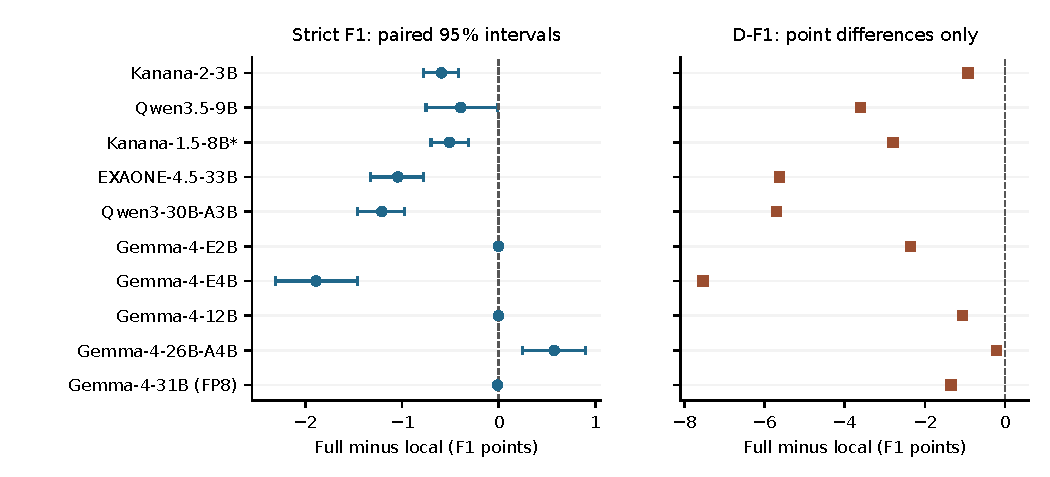
\includegraphics[width=\textwidth]{figures/context-contrasts.pdf}
\caption{Within-model full-minus-local contrasts on each model's original
cohort. Negative values favor local context. Left: strict F1 and pointwise
95\% document-paired bootstrap intervals (2,000 draws, seed 0). Right:
D-F1 point differences; no diagnostic confidence intervals are implied.
*Kanana-1.5-8B uses 1,438 documents; other pairs use 1,440. These are
post-hoc within-model comparisons, not an all-model common-capacity ranking.}
\Description{Two aligned panels show strict F1 differences with intervals
and diagnostic F1 point differences for ten models. Nine strict differences
and all ten diagnostic differences favor local context. Gemma-26B-A4B is
the strict exception. The intervals for Gemma-E2B and Gemma-12B cross zero.}
\label{fig:context-contrasts}
\end{figure*}

\section{Output Diagnostics and Reproducibility}
\label{app:diagnostics}

All scores use the frozen preview and preserve the original strict results. There are 22 completed LLM conditions and three frozen baselines; no pilot or partial scores enter the tables. Each 1,440-document LLM run comprises 13,723 requests and 218,664 gold mentions. Kanana-1.5-8B uses 1,438 documents, 13,653 requests and 218,197 mentions after two recorded length exclusions. No missing pair is imputed. The comparison is an archival completed-run study, not evidence that every originally planned experiment completed.

\paragraph{Serving and sampling.}
Operator records report vLLM 0.30.0 for Qwen/Kanana/EXAONE (BF16, temperature 1, top-$p$ 1), and vLLM 0.19.0 for Gemma on one H100 80GB. Gemma inherits its native generation settings (temperature 1, top-$p$ 0.95, top-$k$ 64); thinking is disabled. Gemma-31B uses FP8 weights and FP8 KV cache, while the other Gemma models use BF16. Gemma's runner dependency inventory differs from its server inventory; these must not be conflated. Archived revisions, request hashes, raw-response hashes, original runner/source hashes and replay-scoring hashes accompany the reproducibility records. Output replay verifies scoring and request coverage, not deployment equivalence. Recorded gate summaries do not independently validate missing native counts. No source stamp was substituted to make external-runner outputs pass a native exporter.

\paragraph{Reading the diagnostic table.}
Table~\ref{tab:response-diagnostics} reports the three diagnostic views
specified in \S\ref{sec:protocol}. Compliance and empty-list rates use all
requests, whereas D scores use all gold and invalid-item penalties. These
columns cannot be multiplied into a single error rate. In particular, an
empty list may be structurally compliant but contribute no true positives.

\begin{table*}[t]
\caption{Post-hoc output diagnostics (0--100). Fmt: structural compliance; Empty: empty-list rate; D: detection proxy. Invalid items incur exact-FP penalties. F/L: full/local; $\dagger$: 1,438 documents.}
\label{tab:response-diagnostics}
\small
\begin{tabular*}{\textwidth}{@{\extracolsep{\fill}}llrrrrrr@{}}
\toprule
System & Context & Fmt & Empty & D-Prc & D-Rec & D-F1 & Invalid items \\
\midrule
Qwen3.5-2B & F & 28.48 & 1.38 & 3.39 & 1.08 & 1.64 & 64,498 \\
Qwen3.5-4B & L & 47.37 & 4.99 & 12.59 & 6.52 & 8.59 & 83,370 \\
Kanana-2-3B & F & 72.22 & 2.18 & 5.64 & 2.20 & 3.17 & 75,465 \\
Kanana-2-3B & L & 63.62 & 8.69 & 12.02 & 2.47 & 4.09 & 31,764 \\
Qwen3.5-9B & F & 75.79 & 16.83 & 18.58 & 11.81 & 14.44 & 96,349 \\
Qwen3.5-9B & L & 76.35 & 13.82 & 22.62 & 15.02 & 18.05 & 87,614 \\
Kanana-1.5-8B$^\dagger$ & F & 46.09 & 0.74 & 5.11 & 6.09 & 5.55 & 235,147 \\
Kanana-1.5-8B$^\dagger$ & L & 40.01 & 0.23 & 12.01 & 6.40 & 8.35 & 83,701 \\
EXAONE-4.5-33B & F & 62.88 & 26.36 & 8.67 & 9.07 & 8.87 & 186,354 \\
EXAONE-4.5-33B & L & 80.13 & 29.86 & 14.68 & 14.33 & 14.50 & 145,380 \\
Qwen3-30B-A3B & F & 90.42 & 53.06 & 9.38 & 6.31 & 7.55 & 123,733 \\
Qwen3-30B-A3B & L & 93.78 & 17.61 & 15.04 & 11.84 & 13.25 & 123,434 \\
Gemma-4-E2B & F & 0.04 & 46.69 & 16.55 & 6.89 & 9.73 & 62,457 \\
Gemma-4-E2B & L & 1.28 & 54.11 & 28.10 & 7.70 & 12.09 & 28,868 \\
Gemma-4-E4B & F & 84.00 & 5.62 & 16.35 & 12.64 & 14.25 & 129,082 \\
Gemma-4-E4B & L & 87.34 & 8.88 & 30.42 & 16.98 & 21.79 & 65,661 \\
Gemma-4-12B & F & 5.55 & 12.19 & 31.94 & 26.15 & 28.76 & 85,401 \\
Gemma-4-12B & L & 5.55 & 7.79 & 30.84 & 28.85 & 29.81 & 92,237 \\
Gemma-4-26B-A4B & F & 95.77 & 12.29 & 34.78 & 24.60 & 28.82 & 69,113 \\
Gemma-4-26B-A4B & L & 96.10 & 7.19 & 31.14 & 27.20 & 29.04 & 84,943 \\
Gemma-4-31B (FP8) & F & 4.98 & 5.74 & 29.00 & 31.59 & 30.24 & 102,275 \\
Gemma-4-31B (FP8) & L & 4.56 & 4.17 & 28.86 & 34.86 & 31.58 & 104,568 \\
\bottomrule
\end{tabular*}
\end{table*}

\subsection{Taxonomy groups and context contrasts}
\label{app:result-layout}

Table~\ref{tab:taxonomy-results} aggregates strict TP/FP/FN within each taxonomy group before computing precision/recall/F1. It does not average category F1. The groups encode our detection policy, not relative legal severity. Stratification by T level, operation, subject role, document type and generator remains available in the archived results. T levels are different documents rather than paired rewrites. Character-overlap diagnostics use valid anchored predictions and all gold, but cannot charge character FP for unanchorable items; interpret them with invalid-item counts and exact penalized precision.

\begin{table*}[t]
\caption{Strict taxonomy-group Prc/Rec/F1 (0--100). F/L: full/local; D: document-level baseline. $\dagger$: 1,438 documents; others 1,440.}
\label{tab:taxonomy-results}
\small
\begin{tabular*}{\textwidth}{@{\extracolsep{\fill}}llrrrrrrrrr@{}}
\toprule
& & \multicolumn{3}{c}{L / identifier} & \multicolumn{3}{c}{L / attribute} & \multicolumn{3}{c}{I / attribute} \\
System & Context & Prc & Rec & F1 & Prc & Rec & F1 & Prc & Rec & F1 \\
\midrule
Qwen3.5-2B & F & 45.23 & 0.13 & 0.25 & 0.00 & 0.00 & 0.00 & 0.00 & 0.00 & 0.00 \\
Qwen3.5-4B & L & 59.04 & 1.04 & 2.05 & 0.00 & 0.00 & 0.00 & 14.02 & 0.02 & 0.05 \\
Kanana-2-3B & F & 60.59 & 1.07 & 2.11 & 12.20 & 0.01 & 0.02 & 17.47 & 0.06 & 0.12 \\
Kanana-2-3B & L & 44.18 & 1.71 & 3.29 & 9.41 & 0.01 & 0.03 & 22.41 & 0.10 & 0.20 \\
Qwen3.5-9B & F & 72.98 & 3.44 & 6.57 & 19.61 & 0.17 & 0.33 & 20.49 & 0.16 & 0.31 \\
Qwen3.5-9B & L & 70.41 & 3.92 & 7.43 & 15.45 & 0.14 & 0.28 & 18.75 & 0.14 & 0.27 \\
Kanana-1.5-8B$^\dagger$ & F & 71.08 & 0.31 & 0.63 & 42.00 & 0.04 & 0.08 & 37.50 & 0.04 & 0.08 \\
Kanana-1.5-8B$^\dagger$ & L & 66.51 & 0.84 & 1.66 & 26.67 & 0.03 & 0.06 & 32.32 & 0.10 & 0.20 \\
EXAONE-4.5-33B & F & 64.57 & 0.70 & 1.39 & 20.31 & 0.22 & 0.43 & 27.09 & 0.11 & 0.21 \\
EXAONE-4.5-33B & L & 69.59 & 1.67 & 3.27 & 44.22 & 0.52 & 1.03 & 30.88 & 0.14 & 0.27 \\
Qwen3-30B-A3B & F & 75.10 & 0.55 & 1.09 & 1.72 & $<0.01$ & $<0.01$ & 20.00 & 0.02 & 0.03 \\
Qwen3-30B-A3B & L & 68.71 & 1.82 & 3.55 & 18.32 & 0.07 & 0.14 & 13.93 & 0.05 & 0.11 \\
Gemma-4-E2B & F & 75.00 & $<0.01$ & 0.01 & 0.00 & 0.00 & 0.00 & 0.00 & 0.00 & 0.00 \\
Gemma-4-E2B & L & 71.43 & $<0.01$ & 0.01 & 0.00 & 0.00 & 0.00 & 14.29 & $<0.01$ & $<0.01$ \\
Gemma-4-E4B & F & 80.99 & 5.45 & 10.21 & 34.74 & 0.60 & 1.18 & 33.82 & 0.36 & 0.72 \\
Gemma-4-E4B & L & 77.97 & 7.37 & 13.47 & 39.09 & 1.02 & 2.00 & 28.50 & 0.54 & 1.05 \\
Gemma-4-12B & F & 70.15 & 0.05 & 0.09 & 0.00 & 0.00 & 0.00 & 0.00 & 0.00 & 0.00 \\
Gemma-4-12B & L & 62.82 & 0.05 & 0.10 & 11.11 & $<0.01$ & $<0.01$ & 0.00 & 0.00 & 0.00 \\
Gemma-4-26B-A4B & F & 71.80 & 9.00 & 15.99 & 12.89 & 0.25 & 0.49 & 9.05 & 0.12 & 0.23 \\
Gemma-4-26B-A4B & L & 71.23 & 8.31 & 14.89 & 8.40 & 0.25 & 0.49 & 8.46 & 0.15 & 0.30 \\
Gemma-4-31B (FP8) & F & 40.00 & $<0.01$ & $<0.01$ & 3.03 & $<0.01$ & $<0.01$ & 6.25 & $<0.01$ & $<0.01$ \\
Gemma-4-31B (FP8) & L & 58.06 & 0.02 & 0.04 & 3.12 & $<0.01$ & $<0.01$ & 0.00 & 0.00 & 0.00 \\
Presidio & D & 64.42 & 11.92 & 20.12 & 0.00 & 0.00 & 0.00 & 0.00 & 0.00 & 0.00 \\
ko-pii & D & 8.67 & 24.95 & 12.87 & 0.00 & 0.00 & 0.00 & 0.01 & $<0.01$ & $<0.01$ \\
OpenMed & D & 9.68 & 2.62 & 4.13 & 0.00 & 0.00 & 0.00 & 0.00 & 0.00 & 0.00 \\
\bottomrule
\end{tabular*}
\end{table*}

\begin{table}[t]
\caption{Within-model strict full-minus-local F1, in points, with pointwise 95\% document-paired bootstrap intervals (2,000 draws, seed 0). Exploratory intervals are not multiplicity-adjusted.}
\label{tab:paired-context}
\small
\begin{tabularx}{\columnwidth}{@{}>{\RaggedRight\arraybackslash}Xrrr@{}}
\toprule
System & $N$ & $\Delta$ & 95\% CI \\
\midrule
Kanana-2-3B & 1440 & -0.593 & [-0.774, -0.413] \\
Qwen3.5-9B & 1440 & -0.393 & [-0.752, -0.015] \\
Kanana-1.5-8B$^\dagger$ & 1438 & -0.509 & [-0.701, -0.313] \\
EXAONE-4.5-33B & 1440 & -1.043 & [-1.322, -0.776] \\
Qwen3-30B-A3B & 1440 & -1.209 & [-1.464, -0.973] \\
Gemma-4-E2B & 1440 & -0.003 & [-0.010, +0.006] \\
Gemma-4-E4B & 1440 & -1.888 & [-2.304, -1.463] \\
Gemma-4-12B & 1440 & -0.003 & [-0.027, +0.023] \\
Gemma-4-26B-A4B & 1440 & +0.573 & [+0.249, +0.899] \\
Gemma-4-31B (FP8) & 1440 & -0.014 & [-0.025, -0.004] \\
\bottomrule
\end{tabularx}
\end{table}

These intervals describe the observed synthetic-document collection and one execution per condition. They do not quantify stochastic rerun variability or population-level production uncertainty. Shared generation plans may induce dependence, and semantic near-duplicate clustering has not been established. The two incomplete Qwen pairs are excluded only from paired analysis, with their completed conditions retained in Table~\ref{tab:main-results}. The medium/large extensions followed qualitative formatting-failure reports; neither model selection nor the diagnostic is preregistered.

\section{Discussion}
\label{sec:discussion}

\paragraph{The extraction contract is part of the measured system.}
The gap between strict and D-F1 exposes a practical distinction: a detector
can emit useful PII spans while failing the interface through which an
application consumes them. Strict rejection measures this deployment-facing
failure, whereas itemwise diagnostics expose the valid evidence remaining
in the same received response. The gap is not an additive estimate of
``performance lost to formatting'': the diagnostic changes both retained
predictions and false-positive accounting, and F1 is nonlinear. Reporting
both scores with compliance, empty-output rates and invalid-item counts
is more informative than selecting whichever score favors a system.

\paragraph{More context is an empirical choice.}
The ten complete pairs consistently favor local context on D-F1, but this
does not establish that financial attributes never require distant evidence.
Full and local conditions share the same explicit target, which may already
contain much of the information needed for the output task. Additional
context can be relevant without improving exact enumeration under a fixed
response budget. Attention dilution, instruction following and output
allocation are possible explanations, not mechanisms identified by these
experiments. Pointwise paired intervals quantify resampling variation over
the observed documents; they do not measure stochastic generation variance
or remove uncertainty about the serving environment.

\paragraph{Coverage matters alongside boundary accuracy.}
Strong identifier performance relative to attribute performance is consistent
with a limited operational coverage of the benchmark policy. It does not
show that contextual attributes are legally less important. Conversely,
an exact-boundary error on a long consultation clause can hide partial
recognition that would be visible under character overlap. The two views
answer different questions: whether the requested typed span was recovered,
and how much labeled text was covered. Character scores cannot charge a
character-level penalty to an unanchorable item and should therefore be
read with invalid-item counts and penalized exact precision. We do not
interpret overlap as a validated measure of remaining disclosure risk.

\paragraph{Implications for financial evaluation.}
These results support evaluating a detector as a policy, an input protocol
and an output contract together. A high format-compliance rate alone does
not show that sensitive information is protected; a low strict score alone
does not locate the failure. The benchmark makes these distinctions
inspectable using the same archived responses. For future deployments,
constrained generation or a different extraction interface would constitute
a new system configuration requiring its own prospective evaluation.
We do not retrofit such changes after observing this test set. The present
study supplies a reproducible characterization of the completed runs,
not a certification that any evaluated system is safe for customer records.

\section{Conclusion and Limitations}
\label{sec:conclusion}

\kiii{} links a traceable Korean financial detection policy to noncanonical inputs and a matched context task. Across completed runs, output-contract failures obscure recoverable PII, while local context consistently improves the post-hoc detection proxy. Reporting strict extraction, structural compliance and all-gold detection together exposes different failure modes without forgiving missed sensitive information.

\paragraph{Limitations and ethics.}
Synthetic documents and practitioner appropriateness review do not establish production representativeness or span correctness. Attribute boundaries may be ambiguous, and semantic near-duplicates have not been audited. T levels are not paired counterfactuals; STT frequencies are design settings. Post-hoc model extensions, decoding/precision differences, unavailable native counts and unverified pilot calibration limit generalization. The diagnostic is an observable proxy, not format-independent ability or legal compliance. No real customer records were used, though coincidental identifier matches remain possible. The preview is CC BY-NC 4.0; a formal release will follow.


\bibliographystyle{ACM-Reference-Format}
\bibliography{references}



\end{document}
